\def\CTeXPreproc{Created by ctex v0.2.9, don't edit!}
%\documentclass{beamer}
\documentclass[%handout,
xcolor=pdftex]{beamer}
\mode<presentation> {
  \usetheme{Warsaw}
  \setbeamercovered{transparent}
}
\let\Tiny=\tiny
\usetheme{Singapore}
\usecolortheme{dolphin}
\usepackage{amsmath}
\usepackage{textcomp}
\usepackage{amssymb}
\usepackage{amsthm}
\usepackage{graphicx}
\usepackage{color}
\usepackage{lipsum}
\usepackage{hyperref}
\usepackage{multirow}
\usepackage{bm}
%\setbeamertemplate{headline}{}
\setbeamertemplate{footline}[page number]
\newcommand\Fontvi{\fontsize{9pt}{8}\selectfont}
\newcommand\Fontvii{\fontsize{7pt}{8}\selectfont}
\newcommand{\backupbegin}{
   \newcounter{finalframe}
   \setcounter{finalframe}{\value{framenumber}}
}
\newcommand{\backupend}{
   \setcounter{framenumber}{\value{finalframe}}
}\newtheorem{proposition}{Proposition}
\title{Unit 13: ARMA Estimation}
\author[STAT 5170: Applied Time Series, Unit 13]{Taylor Brown}
\institute{Department of Statistics, University of Virginia}
\date{Fall 2020}

\AtBeginSubsection[] {
  \begin{frame}<beamer>{Outline}
    \tableofcontents[currentsection,currentsubsection]
  \end{frame}
}

\begin{document}


\frame{\titlepage}


\begin{frame}
\frametitle{Readings for Unit 13}

Textbook chapter 3.5 (pages 115 to 121).

\end{frame}



\begin{frame}
\frametitle{Last Unit}
\begin{enumerate}
\item ARMA forecasting.
\item Prediction error.
\item Prediction interval.
\end{enumerate}
\end{frame}

\begin{frame}
\frametitle{This Unit}
\begin{enumerate}
\item Method of Moments Estimation.
\item Maximum Likelihood Estimation.
\end{enumerate}
\end{frame}


\begin{frame}
\frametitle{Motivation}

In this unit, we explore a couple of ways to estimate the parameters for ARMA models: Method of Moments (MOM) estimation and Maximum Likelihood (ML) estimation.

\end{frame}

\section{Method of Moments Estimation}
\frame{\tableofcontents[currentsection]}

%
%
%\begin{frame}
%\frametitle{ARMA Estimation}
%
%Let's assume that we have a causal and intvertible ARMA model
%$$
%\phi(B)  X_t = \theta(B) w_t,
%$$
%where the white noise $w_t$ has variance $\sigma^2_w$,
%$$
%\phi(B) = 1-\phi_1 B - \cdots - \phi_p B^p \quad
%\mbox{and} \quad
%\theta(B) = 1+\theta_1 B + \cdots+\theta_q B^q.
%$$
%Given $n$ observations $x_1,x_2,\ldots,x_n$, we are interested
%in estimating the parameters
%$\phi_1,\ldots,\phi_p,\theta_1,\ldots,\theta_q$ and
%$\sigma^2_w$. Initially we assume that the orders $p$ and $q$
%are known.
%\end{frame}
%



\begin{frame}
\frametitle{Method of Moments}

Let's start with the method of moments (MOM) estimation. The idea behind this is to equate population moments to sample moments and then solve for the parameters in terms of the sample moments.
\newline

We re-use a lot of the same equations from the previous section!

\end{frame}


\begin{frame}
\frametitle{AR Estimation}

Let's first assume that we have a causal AR(p) model
$$
\phi(B)  (x_t - \mu) = w_t,
$$
where the white noise $w_t$ has variance $\sigma^2_w$,
$$
\phi(B) = 1-\phi_1 B - \cdots - \phi_p B^p .
$$
Given $n$ observations $x_1,x_2,\ldots,x_n$, we are interested in estimating the parameters $\phi_1,\ldots,\phi_p$ and $\sigma^2_w$. Initially we assume that the order $p$ is known.
\end{frame}

\begin{frame}
\frametitle{AR Estimation}

We'll assume again without loss of generality (WLOG) that $\mu = 0$. Why?
\newline

$E[x_t] = \mu$ can always be estimated with the first sample moment $\bar{x}$. 
\newline

If $\mu \neq 0$, then transform your data before estimating as follows:
$\tilde{x}_t = x_t - \bar{x}$.
\end{frame}



\begin{frame}
\frametitle{Yule-Walker Estimation for AR(p)}

The method of moments works well when estimating causal AR(p) models. We consider the causal AR($p$) model
\begin{eqnarray}\label{eq:1}
x_t= \phi_1 x_{t-1} + \cdots + \phi_p x_{t-p} + w_t.
\end{eqnarray}

For $h=1,\ldots,p$, multiply both sides of (\ref{eq:1}) by $x_{t-h}$, and take expectations:

\begin{eqnarray}\label{eq:2}
\gamma(h)  = \phi_1 \gamma(h-1) + \cdots + \phi_p \gamma(h-p)
\end{eqnarray}

When $h=0$, we do the same thing and get
\begin{eqnarray}
\sigma^2_w  = \gamma(0) - \phi_1 \gamma(1) + \cdots + \phi_p \gamma(p)
\end{eqnarray}

\end{frame}


\begin{frame}
\frametitle{Yule-Walker Estimation for AR(p)}

We call these the \textbf{Yule-Walker equations}

\begin{eqnarray*}
\gamma(h) &=&  \phi_1 \gamma(h-1) + \phi_2 \gamma(h-2) + \cdots + \phi_p \gamma(h-p), \hspace{5mm} h=1,\ldots,p  \\
\sigma_{w}^2 &=& \gamma(0) - \phi_1 \gamma(1) - \phi_2 \gamma(2) - \cdots - \phi_p \gamma(p).
\end{eqnarray*}

We can also write them in matrix notation that should look familiar:
$$
\Gamma_p \phi = \gamma_p \hspace{10mm} \sigma^2_w = \gamma(0) - \phi' \gamma_p
$$

where $\Gamma_p = \{\gamma(k-j) \}_{j,k=1}^p$ is a $p \times p$ matrix, $\phi = (\phi_1, \cdots, \phi_p)^{\prime}$ is a $p \times 1$ vector, and $\gamma_p = (\gamma(1), \cdots, \gamma(p))^{\prime}$ is a $p \times 1$ vector.


\end{frame}


\begin{frame}
\frametitle{Yule-Walker Estimation for AR(p)}

Using method of moments, put hat signs on everything, and then solve for the desired parameters:
$$
\Gamma_p \phi = \gamma_p \hspace{10mm} \sigma^2_w = \gamma(0) - \phi' \gamma_p
$$
yields
\begin{equation*}
\hat{\phi} = \hat{\Gamma}_p^{-1} \hat{\gamma}_p
\end{equation*}

and

\begin{equation*}
\hat{\sigma}_w^2 = \hat{\gamma}(0) - \hat{\gamma}_p^{\prime} \hat{\Gamma}_p^{-1} \hat{\gamma}_p.
\end{equation*}

\end{frame}

\begin{frame}
\frametitle{Yule-Walker Estimation for AR(p)}

One more small move: divide through by $\hat{\gamma}(0)$ before solving, so that we have formulas in terms of ACFs.
\newline

$$
\frac{1}{\gamma(0)} \Gamma_p \phi = \frac{1}{\gamma(0)}\gamma_p \hspace{10mm} \sigma^2_w = \gamma(0) - \phi' \gamma_p
$$
gives us

\begin{equation} \label{eq:s1}
\hat{\phi} = \hat{R}_p^{-1} \hat{\rho}_p
\end{equation}

and

\begin{eqnarray} \label{eq:s2}
\hat{\sigma}_w^2 &=& \hat{\gamma}(0) \left[ 1 - \hat{\rho}_p^{\prime} \hat{R}_p^{-1} \hat{\rho}_p \right] \nonumber 
\end{eqnarray}
%\\
%                 &=& \hat{\gamma}(0) \left[ 1 - \hat{\boldsymbol{\rho}}_p^{\prime} \boldsymbol{\hat{\phi}} \right],

where $\hat{R}_p = \{\hat{\rho}(k-j) \}_{j,k=1}^p$ is a $p \times p$ matrix and $\hat{\rho}_p = (\hat{\rho}(1), \cdots, \hat{\rho}(p))^{\prime}$ is a $p \times 1$ vector.

\end{frame}

\begin{frame}
\frametitle{Yule-Walker Estimation for AR(p)}

The asymptotic behavior of the Yule-Walker estimators for causal AR(p) processes is

\begin{equation} \label{eq:asymp}
\sqrt{n}\left(\hat{\bm{\phi}} - \bm{\phi}\right) \xrightarrow[]{d} N\left( \bm{0}, \sigma_w^2 \bm{\Gamma}_p^{-1} \right)
\end{equation}

and

\begin{equation*}
\hat{\sigma}_w^2 \xrightarrow[]{p} \sigma_w^2.
\end{equation*}

\end{frame}

\begin{frame}
\frametitle{Yule-Walker Estimation for AR(p)}

The variance-covariance matrix for $\hat{\bm{\phi}}$ is

\begin{eqnarray} \label{eq:varmatrix}
Var(\hat{\bm{\phi}}) &=& \frac{\sigma^2}{n} \bm{\Gamma}_p^{-1} \nonumber \\
                     &=& \frac{\sigma^2}{n\hat{\gamma}(0)}  \bm{R}_p^{-1}
\end{eqnarray}

\end{frame}


\begin{frame}[fragile]
\frametitle{Simulation Example}

Using the \verb=armasim()= function, I simulated $n=1000$ observations from the following AR(2) process

$$
x_t = 1.5 x_{t-1} - 0.75 x_{t-2} + w_t
$$

where $\sigma_w^2 = 1$. For the sample, $\hat{\gamma}(0) = 7.69697$, $\hat{\rho}(1)=0.8456375$, and $\hat{\rho}(2) = 0.5054795$.

\end{frame}

\begin{frame}
\frametitle{Simulation Example}

The data had $\hat{\rho}(1) = .849$, $\hat{\rho}(2) = .519$ and $\hat{\gamma}(0) = 8.903$
\begin{align*}
\hat{\phi} &= \hat{R}_p^{-1} \hat{\rho}_p \\
&= \begin{bmatrix}
1 & .849 \\
.849 & 1
\end{bmatrix}^{-1}
\begin{bmatrix}
.849 \\
.519
\end{bmatrix} \\
&= 
\begin{bmatrix}
1.463 \\
-.723
\end{bmatrix}
\end{align*}

Also, 
\begin{align*}
\hat{\sigma}_w^2 &= \hat{\gamma}(0) \left[ 1 - \hat{\rho}_p^{\prime} \hat{R}_p^{-1} \hat{\rho}_p \right] \\
&= \hat{\gamma}(0) \left[ 1 - \hat{\rho}_p^{\prime} \hat{\phi} \right] \\
&=  8.903 * (1 - \begin{bmatrix} .849 & .519 \end{bmatrix} \begin{bmatrix} 1.463 \\ -.723\end{bmatrix}) = 1.187
\end{align*}
\end{frame}




\begin{frame}
\frametitle{Fish Population Example}

In Unit 11, we looked at the ACF and PACF of the time series from ``recruit.dat", which contains data on fish population in the central Pacific Ocean. The numbers represent the number of new fish for each month in the years 1950-1987. 
\end{frame}

\begin{frame}
\frametitle{Fish Population Example}

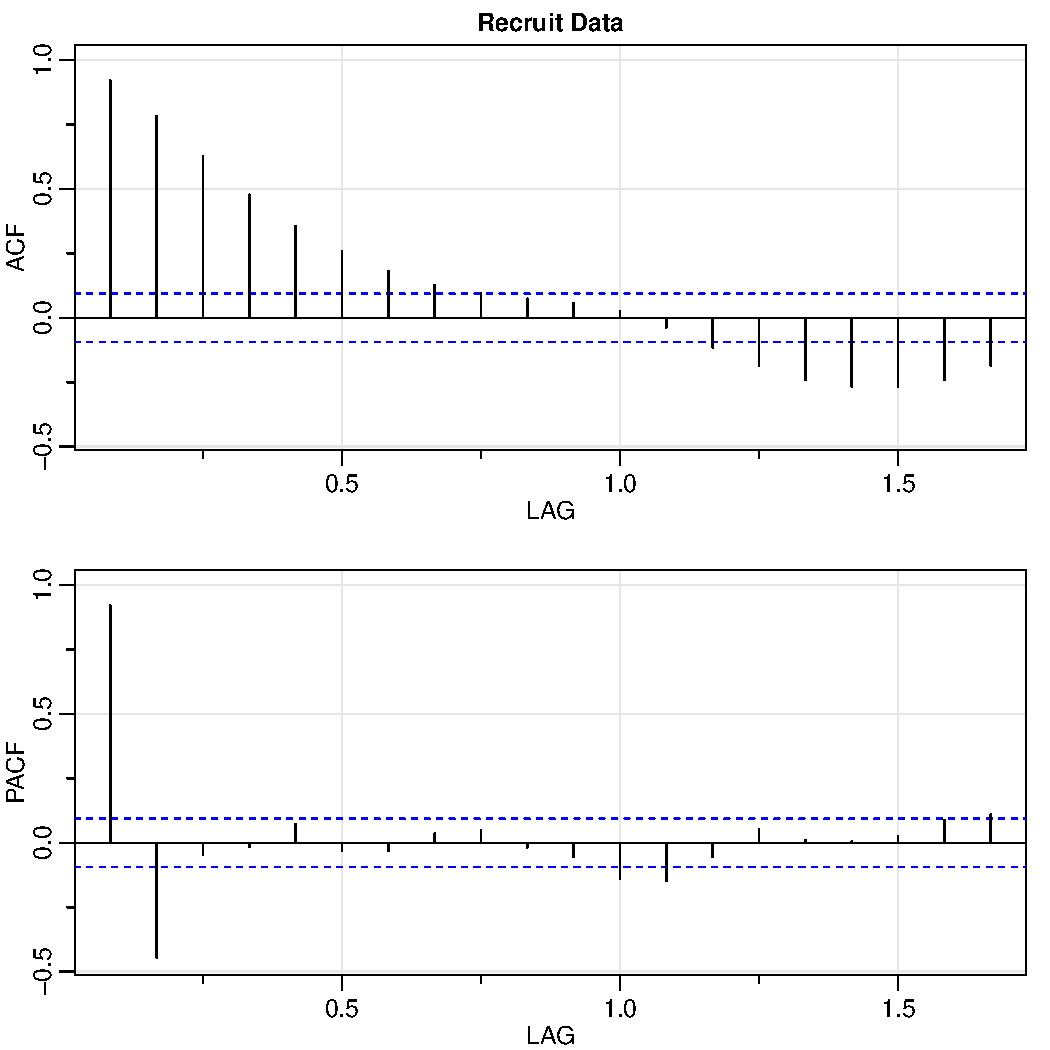
\includegraphics[width=100mm, height=80mm]{recruit.pdf}

\end{frame}


\begin{frame}[fragile]
\frametitle{Fish Population Example}

Let's check the results of fitting an AR(2) model using Yule-Walker estimation in R.

\begin{verbatim}
> rec.yw<-ar.yw(rec, order=2)
> rec.yw$x.mean
[1] 62.26278
> rec.yw$ar
[1]  1.3315874 -0.4445447
> sqrt(diag(rec.yw$asy.var.coef))
[1] 0.04222637 0.04222637
\end{verbatim}

\end{frame}

\begin{frame}
\frametitle{Fish Population Example}

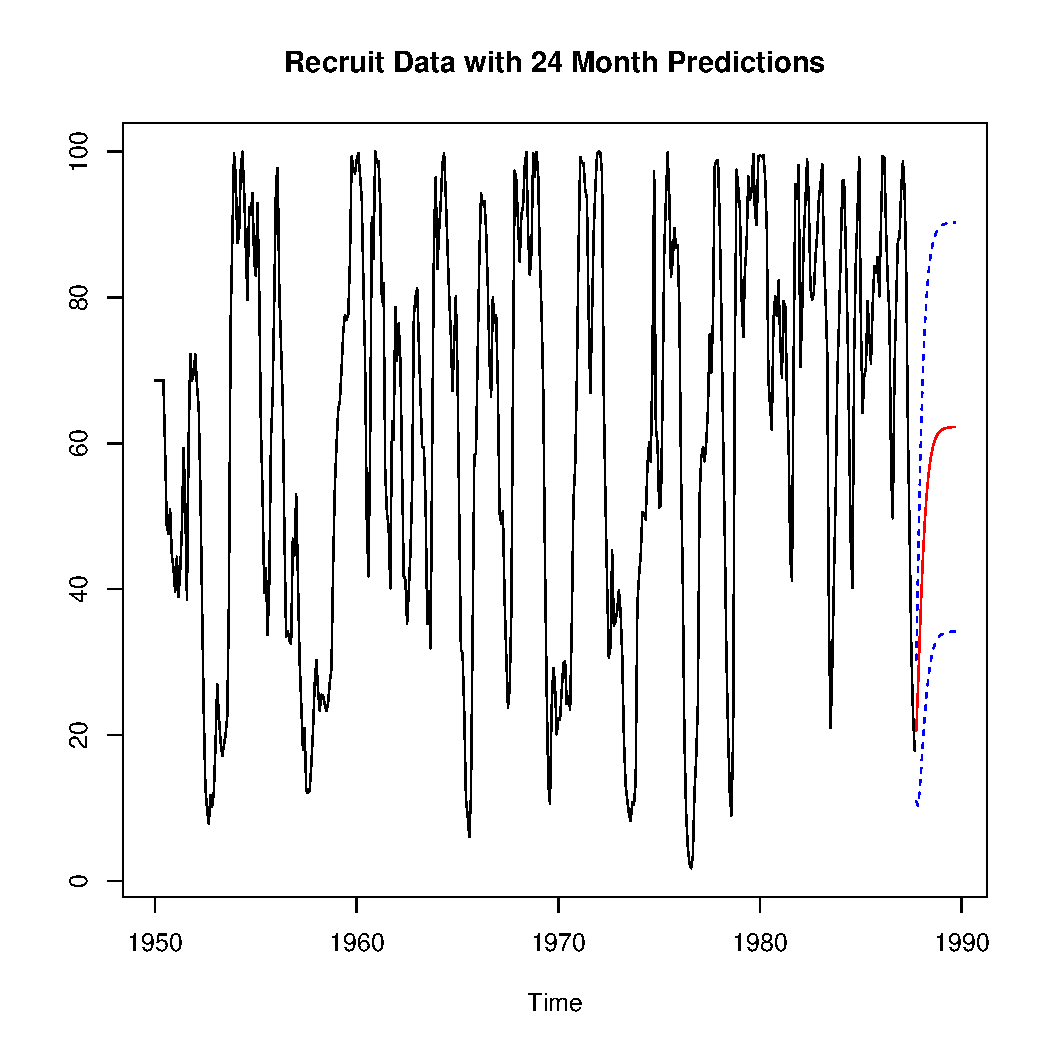
\includegraphics[width=100mm, height=80mm]{pred.pdf}

\end{frame}

\begin{frame}[fragile]
\frametitle{Fish Population Example}

\begin{verbatim}
rec.pred <- predict(rec.yw, n.ahead=24)
ts.plot(rec, rec.pred$pred, col=1:2)
lines(rec.pred$pred - rec.pred$s, col=4, lty=2)
lines(rec.pred$pred + rec.pred$s, col=4, lty=2)
\end{verbatim}

\end{frame}

\begin{frame}
\frametitle{Method of Moments Estimation for MA(q)}

Consider an invertible MA(1) process $x_t = w_t + \theta w_{t-1}$, with $|\theta| < 1$. We know that

$$
\rho(1) = \frac{\theta}{1 + \theta^2}.
$$

Using method of moments, we equate $\hat{\rho}(1)$ to $\rho(1)$ and solve a quadratic equation in $\theta$.


\end{frame}

\begin{frame}
\frametitle{Method of Moments Estimation for MA(q)}

The invertible solution(s) is(are)

$$
\hat{\theta} = \frac{1 \pm \sqrt{1 - 4 \hat{\rho}(1)^2}}{2 \hat{\rho}(1)}.
$$
\begin{itemize}
\item If $|\hat{\rho}(1)| < 0.5$, two solutions exist, so we pick the invertible one. 
\item If $\hat{\rho}(1)= \pm 0.5$, $\hat{\theta} = \pm 1$. No invertible solution. 
\item If $\hat{\rho}(1)>0.5$, no real solutions exist: the method of moments fails to yield an estimator of $\theta$.
\end{itemize}

\end{frame}

\begin{frame}
\frametitle{Method of Moments Estimation for MA(q)}

For higher order MA(q) models, the method of moments quickly gets complicated. The equations are non-linear in $\theta_1, \cdots, \theta_q$, so numerical methods need to be used. 

\end{frame}

\section{Maximum Likelihood Estimation}
\frame{\tableofcontents[currentsection]}

\begin{frame}
\frametitle{Maximum Likelihood Estimation}

To illustrate the main concept with maximum likelihood estimation, we consider the AR(1) model with nonzero mean

\begin{eqnarray}\label{eq:ar1}
x_t=\mu+\phi(x_{t-1}-\mu)+w_t,
\end{eqnarray}

where $|\phi|<1$ and $w_t\sim iid $ N(0,$\sigma^2_w$).

\end{frame}

\begin{frame}
\frametitle{Maximum Likelihood Estimation}

We seek the likelihood
\begin{eqnarray}\label{eq:likelihood}
L(\mu,\phi,\sigma^2_w) = f_{\mu,\phi,\sigma^2_w}(x_1,x_2,\ldots,x_n).
\end{eqnarray}
The likelihood function (\ref{eq:likelihood}) $L(\mu,\phi,\sigma^2_w)$ is functionally equivalent to the joint probability distribution of the observed data $x_1,x_2,\ldots,x_n$. 

\end{frame}

\begin{frame}
\frametitle{Maximum Likelihood Estimation}

For a given data set, think of the likelihood as a function of the parameters (not the data). Since we've already observed the data $x_1,x_2,\ldots,x_n$, we
can find parameters $(\mu,\phi,\sigma^2_w)$ to maximize the likelihood $L(\mu,\phi,\sigma^2_w)$. This is the basic idea behind maximum likelihood estimation.

\end{frame}


\begin{frame}
\frametitle{Likelihood Function}

We will use the following:
\begin{align*}
L(\mu,\phi,\sigma^2_w) &= f(x_1, \ldots, x_t) \\
&= f(x_1) f(x_2 | x_1) f(x_3 | x_2, x_1) \cdots f(x_t | x_{t-1}, x_{t-2}, \ldots, x_1) \\
&= f(x_1) f(x_2 | x_1) f(x_3 | x_2) \cdots f(x_t | x_{t-1}) 
\end{align*}


\end{frame}

\begin{frame}
\frametitle{Likelihood Function}

These are all the same:
$$
x_t =\mu+\phi(x_{t-1}-\mu) + w_t \hspace{5mm} w_t \sim \text{Normal}(0, \sigma^2_w)
$$

\begin{eqnarray*}
x_t|x_{t-1}  \sim \text{Normal}(\mu+\phi(x_{t-1}-\mu),\sigma^2_w)
\end{eqnarray*}
and
\begin{eqnarray*}
 f_{x_t|x_{t-1}}(x_t|x_{t-1}) = \frac{1}{\sqrt{2\pi \sigma_w^2}}
\exp \Big \{-\frac{[x_t-\mu-\phi(x_{t-1}-\mu)]^2}{2\sigma^2 _w} \Big \}.
\end{eqnarray*}


\end{frame}

%\begin{frame}
%\frametitle{Likelihood Function}
%
%Similarly,
%\begin{eqnarray*}
%f_{x_t|x_{t-1}}(x_t|x_{t-1}) = \frac{1}{\sqrt{2\pi \sigma_w^2}}
%\exp \Big \{-\frac{[x_t-\mu-\phi(x_{t-1}-\mu)]^2}{2\sigma^2 _w} \Big \}.
%\end{eqnarray*}
%
%\end{frame}

\begin{frame}
\frametitle{Likelihood Function}

We have
\begin{align*}\label{eq:cle}
L(\mu,\phi,\sigma^2_w) &= f_{x_1}(x_1) \times f_{x_2|x_1}(x_2|x_1) \times \cdots \times f_{x_n|x_{n-1}}(x_n|x_{n-1}) \cr \\
&= f_{x_1}(x_1) (2\pi \sigma^2_w)^{-(n-1)/2} \times \\
&\hspace{10mm}\exp \Big \{ -\frac{ \sum^n_{t=2} [x_t-\mu-\phi(x_{t-1}-\mu)]^2 }{2\sigma^2_w} \Big \}.
\end{align*}

\end{frame}


\begin{frame}
\frametitle{Likelihood Function: what is $f_{x_1}(x_1)$?}

In midterm 1, we assumed 
$$
x_1 \sim \text{Normal}\left(\mu, \frac{\sigma^2}{1-\phi^2} \right)
$$
because that would allow all other time points to have the same marginal distribution.
\newline

Here's another rationalization: assume this model is causal ($|\phi|<1$), and pretend you have an infinite history of data (impossible in practice).
\newline

The causal representation $x_1=\mu+\sum^\infty_{j=0} \phi^j
w_{1-j}$ is. Take expectations on both sides, and take the variance on both sides. 
\newline

Since $w_t$ are iid normal, $x_1$ is a normal with mean $\mu$ and variance $\sigma^2_w/(1-\phi^2)$.

%, and
%\begin{eqnarray*}
%f_{x_1}(x_1)=\frac{1}{\sqrt{2\pi \sigma^2_w/(1-\phi^2)}}
%\exp \Big \{- \frac{(x_1-\mu)^2}{2\sigma^2_w/(1-\phi^2)} \Big \}
%\end{eqnarray*}

\end{frame}

\begin{frame}
\frametitle{Likelihood Function}

The likelihood function is
\begin{align*}
L(\mu,\phi,\sigma^2_w) &= f_{x_1}(x_1) (2\pi \sigma^2_w)^{-(n-1)/2} \exp \Big \{ -\frac{ \sum^n_{t=2} [x_t-\mu-\phi(x_{t-1}-\mu)]^2 }{2\sigma^2_w} \Big \}\\
&= (2\pi \sigma^2_w)^{-n/2}(1 - \phi^2)^{1/2} \exp \Big \{ -\frac{ S(\mu,\phi) }{2\sigma^2_w} \Big \},
\end{align*}
where
\begin{eqnarray*}
S(\mu,\phi) = (1-\phi^2)(x_1 - \mu)^2 \sum^n_{t=2} [x_t-\mu-\phi(x_{t-1}-\mu)]^2.
\end{eqnarray*}

\end{frame}




%
%\begin{frame}
%\frametitle{Likelihood Function}
%
%Thus, for given data $x_1,x_2,\ldots,x_n$, we can find
%$(\mu,\phi,\sigma^2_w)$ to maximize the likelihood
%$L(\mu,\phi,\sigma^2_w)$. 
%
%It is worth pointing out that it is more common to consider the log-likelihood
%\begin{eqnarray*}
%\ell(\mu,\phi,\sigma^2) = \log L(\mu,\phi,\sigma^2).
%\end{eqnarray*}
%
%Maximizing log-likelihoods may not always have a closed-form solution. \textbf{Numerical methods} (e.g.: Newton-Raphson, Fisher scoring) are needed.
%
%\end{frame}


\begin{frame}
\frametitle{The Log-likelihood Function}

It is worth pointing out that it is more common to consider the log-likelihood
\begin{align*}
\ell(\mu,\phi,\sigma^2) &= \log L(\mu,\phi,\sigma^2) \\
&= \log \left[ (2\pi \sigma^2_w)^{-n/2}(1 - \phi^2)^{1/2} \exp \Big \{ -\frac{ S(\mu,\phi) }{2\sigma^2_w} \Big \} \right] \\
&= -\frac{n}{2} \log (2\pi \sigma^2_w) + \frac{1}{2}\log (1 - \phi^2) -\frac{ S(\mu,\phi) }{2\sigma^2_w} 
\end{align*}

Numerically more stable, and the derivatives are easier to calculate.
%Maximizing log-likelihoods may not always have a closed-form solution. \textbf{Numerical methods} (e.g.: Newton-Raphson, Fisher scoring) are needed.

\end{frame}


\begin{frame}
\frametitle{The variance estimator}

The variance estimator can be obtained after you get the other estimators:
\begin{align*}
\frac{d}{d\sigma^2}L(\mu,\phi,\sigma^2_w) &= \frac{d}{d\sigma^2}\left[-\frac{n}{2} \log (2\pi \sigma^2_w) + \frac{1}{2}\log (1 - \phi^2) -\frac{ S(\mu,\phi) }{2\sigma^2_w} \right]\\
&= -\frac{n}{2 \sigma^2_w} +  S(\mu,\phi)\left(\frac{1}{\sigma^2_w}\right)^2 
\end{align*}

Setting that equal to $0$, replacing $\sigma^2_w$ with $\hat{\sigma}^2_w$, and solving for $\hat{\sigma}^2_w$ gives us
$$
\hat{\sigma}^2_w = \frac{S(\mu,\phi)}{n}
$$

\end{frame}


\begin{frame}
\frametitle{The variance estimator}

The estimates for $\mu$ and $\sigma^2$ is more complicated. Taking the derivative with respect to these, and setting the equations equal to $0$ yields something that cannot be solved analytically. It's usually accomplished with a numerical procedure (e.g. Newton-Raphson or Fisher scoring).

\end{frame}


\section{Comparison of MOM and MLE}
\frame{\tableofcontents[currentsection]}


\begin{frame}
\frametitle{Properties of ML Estimators}

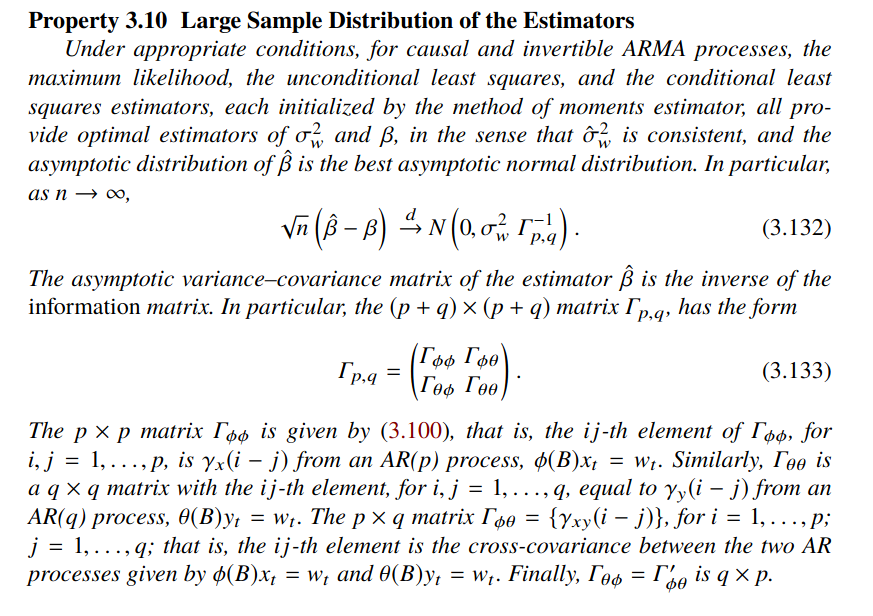
\includegraphics[width=100mm]{screenshot.png}

\end{frame}



\end{document} 